\documentclass{report}
% Include all project wide packages here.
\usepackage{fullpage}
\usepackage{polyglossia}
\setmainlanguage{dutch}
\usepackage{csquotes}
\usepackage{graphicx}
\usepackage{epstopdf}
\usepackage{pdfpages}
\usepackage{caption}
\usepackage[list=true]{subcaption}
\usepackage{float}
%\usepackage{mathtools}
\usepackage{standalone}
\usepackage{import}
\usepackage{tocloft}
\usepackage{wrapfig}
\usepackage{authblk}
\usepackage{array}
\usepackage{booktabs}
\usepackage[toc,page,title,titletoc]{appendix}
\usepackage{xunicode}
\usepackage{amsmath}
\usepackage{fontspec}
\usepackage{unicode-math}
\usepackage[
    backend=bibtexu,
	texencoding=utf8,
bibencoding=utf8,
    style=ieee,
    sortlocale=nl_NL,
    language=auto
]{biblatex}
\usepackage{listings}
\newcommand{\includecode}[3][c]{\lstinputlisting[caption=#2, escapechar=, style=#1]{#3}}
\newcommand{\superscript}[1]{\ensuremath{^{\textrm{#1}}}}
\newcommand{\subscript}[1]{\ensuremath{_{\textrm{#1}}}}


\newcommand{\chapternumber}{\thechapter}
\renewcommand{\appendixname}{Bijlage}
\renewcommand{\appendixtocname}{Bijlagen}
\renewcommand{\appendixpagename}{Bijlagen}

\usepackage[hidelinks]{hyperref} %<--------ALTIJD ALS LAATSTE

%\renewcommand{\familydefault}{\sfdefault}

\setmainfont[Ligatures=TeX]{Myriad Pro}
\setmathfont{Asana Math}
\setmonofont{Lucida Console}

\usepackage{titlesec, blindtext, color}
\definecolor{gray75}{gray}{0.75}
\newcommand{\hsp}{\hspace{20pt}}
\titleformat{\chapter}[hang]{\Huge\bfseries}{\chapternumber\hsp\textcolor{gray75}{|}\hsp}{0pt}{\Huge\bfseries}
\renewcommand{\familydefault}{\sfdefault}
\renewcommand{\arraystretch}{1.2}
\setlength\parindent{0pt}

%For code listings
\definecolor{black}{rgb}{0,0,0}
\definecolor{browntags}{rgb}{0.65,0.1,0.1}
\definecolor{bluestrings}{rgb}{0,0,1}
\definecolor{graycomments}{rgb}{0.4,0.4,0.4}
\definecolor{redkeywords}{rgb}{1,0,0}
\definecolor{bluekeywords}{rgb}{0.13,0.13,0.8}
\definecolor{greencomments}{rgb}{0,0.5,0}
\definecolor{redstrings}{rgb}{0.9,0,0}
\definecolor{purpleidentifiers}{rgb}{0.01,0,0.01}


\lstdefinestyle{csharp}{
language=[Sharp]C,
showspaces=false,
showtabs=false,
breaklines=true,
showstringspaces=false,
breakatwhitespace=true,
escapeinside={(*@}{@*)},
columns=fullflexible,
commentstyle=\color{greencomments},
keywordstyle=\color{bluekeywords}\bfseries,
stringstyle=\color{redstrings},
identifierstyle=\color{purpleidentifiers},
basicstyle=\ttfamily\small}

\lstdefinestyle{c}{
language=C,
showspaces=false,
showtabs=false,
breaklines=true,
showstringspaces=false,
breakatwhitespace=true,
escapeinside={(*@}{@*)},
columns=fullflexible,
commentstyle=\color{greencomments},
keywordstyle=\color{bluekeywords}\bfseries,
stringstyle=\color{bluestrings},
identifierstyle=\color{purpleidentifiers}
}

\lstdefinestyle{vhdl}{
language=VHDL,
showspaces=false,
showtabs=false,
breaklines=true,
showstringspaces=false,
breakatwhitespace=true,
escapeinside={(*@}{@*)},
columns=fullflexible,
commentstyle=\color{greencomments},
keywordstyle=\color{bluekeywords}\bfseries,
stringstyle=\color{redstrings},
identifierstyle=\color{purpleidentifiers}
}

\lstdefinestyle{xaml}{
language=XML,
showspaces=false,
showtabs=false,
breaklines=true,
showstringspaces=false,
breakatwhitespace=true,
escapeinside={(*@}{@*)},
columns=fullflexible,
commentstyle=\color{greencomments},
keywordstyle=\color{redkeywords},
stringstyle=\color{bluestrings},
tagstyle=\color{browntags},
morestring=[b]",
  morecomment=[s]{<?}{?>},
  morekeywords={xmlns,version,typex:AsyncRecords,x:Arguments,x:Boolean,x:Byte,x:Char,x:Class,x:ClassAttributes,x:ClassModifier,x:Code,x:ConnectionId,x:Decimal,x:Double,x:FactoryMethod,x:FieldModifier,x:Int16,x:Int32,x:Int64,x:Key,x:Members,x:Name,x:Object,x:Property,x:Shared,x:Single,x:String,x:Subclass,x:SynchronousMode,x:TimeSpan,x:TypeArguments,x:Uid,x:Uri,x:XData,Grid.Column,Grid.ColumnSpan,Click,ClipToBounds,Content,DropDownOpened,FontSize,Foreground,Header,Height,HorizontalAlignment,HorizontalContentAlignment,IsCancel,IsDefault,IsEnabled,IsSelected,Margin,MinHeight,MinWidth,Padding,SnapsToDevicePixels,Target,TextWrapping,Title,VerticalAlignment,VerticalContentAlignment,Width,WindowStartupLocation,Binding,Mode,OneWay,xmlns:x}
}

%defaults
\lstset{
basicstyle=\ttfamily\small,
extendedchars=false,
numbers=left,
numberstyle=\ttfamily\tiny,
stepnumber=1,
tabsize=4,
numbersep=5pt
}


\begin{document}
\newcommand{\tss}{\textsubscript}
\section{Beschrijving}
De resultaten van het onderzoek, dat hierboven beschreven wordt, bestaan vooral uit grafieken, waaruit een juiste waarde voor C\tss{g} wordt afgelezen. Die grafiek wordt verkregen door de formule (blz 109 uit het boek van Rabae [1])
\begin{equation}
I = C_g(V\tss{GS}) \frac{dV\tss{GS}}{dt}
\end{equation}
om te schrijven naar:
\begin{equation}
C_g(V\tss{GS})= \frac{I}{ \frac{dV\tss{GS}}{dt}}
\end{equation}
Deze functie kun je uit laten rekenen door SPICE. Dan komt er de volgende grafiek uit: (figuur \ref{res:1}) \newline
\begin{figure} [h!]
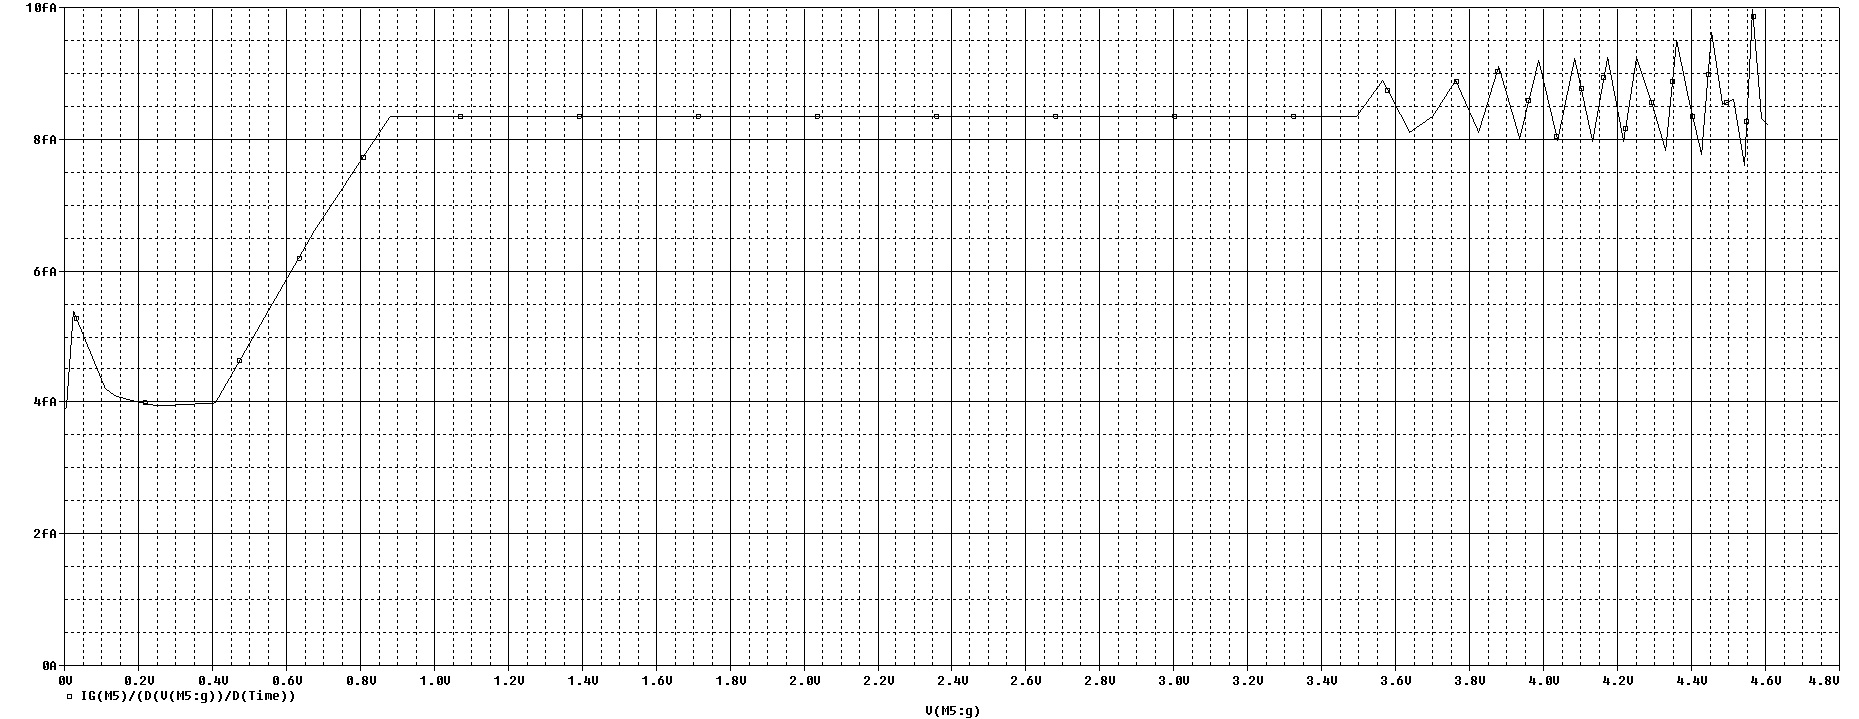
\includegraphics [width = \textwidth] {../figures/nmos/C_L_2_2}
\caption{$C_g$ als functie van V\tss{GS} met W=3um en L = 2.2um.}
\label{res:1}
\end{figure}
Vervolgens kun je SPICE de capaciteit laten bepalen. Dit is het vlakke deel van de grafiek in figuur \ref{res:1}. Zowel voor  de NMOS als voor de PMOS is dit gedaan voor verschillende waarden van L. De strategie is hierboven al beschreven, maar de formule voor de totale gate capaciteit verduidelijkt veel. Deze komt uit de projectopdracht. 
\begin{equation} \label{res:eq1}
C_g = W *c_0 + L *W *C\tss{GC}
\end{equation}
Wanneer W vastgezet en L gevarieerd wordt, verkrijgt met een lineair verband. Voor dezelfde waardes van W en bij verschillende waardes van L is steeds de totale capaciteit bepaald. De resulaten voor zowel de NMOS als de PMOS transistor staan in figuur \ref{res:2}.
\begin{figure} [h!]
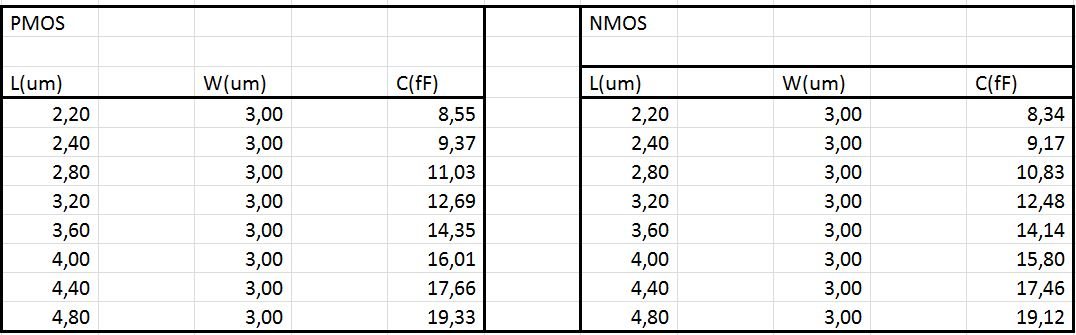
\includegraphics [scale = 0.4] {../figures/tabel}
\caption{De door SPICE berekende waarden van $C_g$ bij veranderende L}
\label{res:2}
\end{figure}
Zoals eerder gezegd, wordt een lineair verband tussen $C_g$ en L verwacht. Wanneer we deze plotten in Matlab (appendix  \ref{M1}) zien we inderdaad een lineair verband, zowel voor de NMOS als voor de PMOS. Met de "Basic Fitting" functie van Matlab werden beide functies bepaald. Die staan onder de figuren \ref{res:3} en \ref{res:4}.

\begin{figure} [h!]
\centering
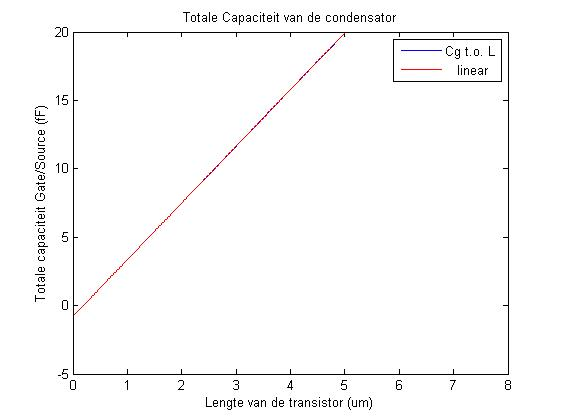
\includegraphics [scale = 0.4] {../figures/c0.jpg}
\caption{$C_g$ vs L, 4.1449x - 0.78078 voor de NMOS}
\label{res:3}
\end{figure}

\begin{figure} [h!]
\centering
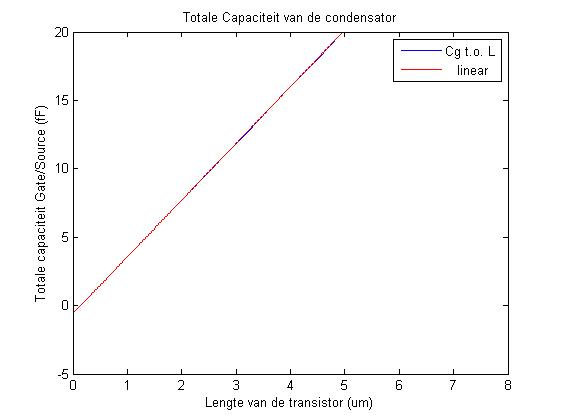
\includegraphics [scale = 0.4] {../figures/c0p.jpg}
\caption{$C_g$ vs L, 4.1464x - 0.57784 voor de PMOS}
\label{res:4}
\end{figure}
Het uiteindelijke doel is om C\tss{GC} te bepalen in vergelijking \ref{res:eq1}. Als je nu de afgeleide naar L neemt, valt de term met $c_0$ eruit:
\begin{equation} \label{res:eq2}
\frac{dC_g}{dL} = \frac{d(W *c_0 + L *W *C\tss{GC})}{dL} = WC\tss{GC} =richtingscoefficient
\end{equation}
De richtingscoëfficient is bepaald met de "basic fitting" functie van Matlab. Uit vergelijking \ref{res:eq2} volgt: 
\begin{equation} \label{res:eq3}
C\tss{GC}= \frac{dC_g}{dL}*\frac{1}{W}
\end{equation}
$\frac{dC_g}{dL}$ is bekend uit de grafiek en W is de vaste waarde die gekozen is. Dan kan C\tss{GC} dus bepaald worden. Hierbij moet vermeld worden dat C\tss{GC} de capaciteit per oppervlakte is. In vergelijking \ref{res:eq3} staat de mogelijkheid om de dikte van het gateoxide te berekenen. Dit is de algemene formule voor een vlakke plaatcondensator.
\begin{equation} \label{res:eq3}
C\tss{GC}*A = \frac { \epsilon \tss{0} \epsilon \tss{r}A } {d}
\end{equation}
Vervolgens kun je de A wegstrepen, waaruit de dikte dan te berekenen is. Om deze dikte snel te kunnen berekenen, is even een matlabcode geschreven. (appendix \ref{M2}). De diktes van de gateoxides van de PMOS en de NMOS staan in tabel \ref{res:tab1}.
\begin{table} [h!]
 \begin{tabular}{ | c |c| } 
\hline
  Dikte gateoxide NMOS (nm) & Dikte gateoxide NMOS (nm) \\ \hline
  30  & 40  \\ \hline
\end{tabular}
\caption{Diktes van gateoxide van de gesimuleerde NMOS en PMOS-transistors}
\label{res:tab1}
 \end{table}
\section{Analyse}
\subsection{Bespreking grafiek in figuur \ref{res:1}}

\subsection{Bespreking uitkomsten}


\end{document}